% Options for packages loaded elsewhere
\PassOptionsToPackage{unicode}{hyperref}
\PassOptionsToPackage{hyphens}{url}
%
\documentclass[
]{article}
\usepackage{amsmath,amssymb}
\usepackage{lmodern}
\usepackage{iftex}
\ifPDFTeX
  \usepackage[T1]{fontenc}
  \usepackage[utf8]{inputenc}
  \usepackage{textcomp} % provide euro and other symbols
\else % if luatex or xetex
  \usepackage{unicode-math}
  \defaultfontfeatures{Scale=MatchLowercase}
  \defaultfontfeatures[\rmfamily]{Ligatures=TeX,Scale=1}
\fi
% Use upquote if available, for straight quotes in verbatim environments
\IfFileExists{upquote.sty}{\usepackage{upquote}}{}
\IfFileExists{microtype.sty}{% use microtype if available
  \usepackage[]{microtype}
  \UseMicrotypeSet[protrusion]{basicmath} % disable protrusion for tt fonts
}{}
\makeatletter
\@ifundefined{KOMAClassName}{% if non-KOMA class
  \IfFileExists{parskip.sty}{%
    \usepackage{parskip}
  }{% else
    \setlength{\parindent}{0pt}
    \setlength{\parskip}{6pt plus 2pt minus 1pt}}
}{% if KOMA class
  \KOMAoptions{parskip=half}}
\makeatother
\usepackage{xcolor}
\usepackage[margin=1in]{geometry}
\usepackage{color}
\usepackage{fancyvrb}
\newcommand{\VerbBar}{|}
\newcommand{\VERB}{\Verb[commandchars=\\\{\}]}
\DefineVerbatimEnvironment{Highlighting}{Verbatim}{commandchars=\\\{\}}
% Add ',fontsize=\small' for more characters per line
\usepackage{framed}
\definecolor{shadecolor}{RGB}{248,248,248}
\newenvironment{Shaded}{\begin{snugshade}}{\end{snugshade}}
\newcommand{\AlertTok}[1]{\textcolor[rgb]{0.94,0.16,0.16}{#1}}
\newcommand{\AnnotationTok}[1]{\textcolor[rgb]{0.56,0.35,0.01}{\textbf{\textit{#1}}}}
\newcommand{\AttributeTok}[1]{\textcolor[rgb]{0.77,0.63,0.00}{#1}}
\newcommand{\BaseNTok}[1]{\textcolor[rgb]{0.00,0.00,0.81}{#1}}
\newcommand{\BuiltInTok}[1]{#1}
\newcommand{\CharTok}[1]{\textcolor[rgb]{0.31,0.60,0.02}{#1}}
\newcommand{\CommentTok}[1]{\textcolor[rgb]{0.56,0.35,0.01}{\textit{#1}}}
\newcommand{\CommentVarTok}[1]{\textcolor[rgb]{0.56,0.35,0.01}{\textbf{\textit{#1}}}}
\newcommand{\ConstantTok}[1]{\textcolor[rgb]{0.00,0.00,0.00}{#1}}
\newcommand{\ControlFlowTok}[1]{\textcolor[rgb]{0.13,0.29,0.53}{\textbf{#1}}}
\newcommand{\DataTypeTok}[1]{\textcolor[rgb]{0.13,0.29,0.53}{#1}}
\newcommand{\DecValTok}[1]{\textcolor[rgb]{0.00,0.00,0.81}{#1}}
\newcommand{\DocumentationTok}[1]{\textcolor[rgb]{0.56,0.35,0.01}{\textbf{\textit{#1}}}}
\newcommand{\ErrorTok}[1]{\textcolor[rgb]{0.64,0.00,0.00}{\textbf{#1}}}
\newcommand{\ExtensionTok}[1]{#1}
\newcommand{\FloatTok}[1]{\textcolor[rgb]{0.00,0.00,0.81}{#1}}
\newcommand{\FunctionTok}[1]{\textcolor[rgb]{0.00,0.00,0.00}{#1}}
\newcommand{\ImportTok}[1]{#1}
\newcommand{\InformationTok}[1]{\textcolor[rgb]{0.56,0.35,0.01}{\textbf{\textit{#1}}}}
\newcommand{\KeywordTok}[1]{\textcolor[rgb]{0.13,0.29,0.53}{\textbf{#1}}}
\newcommand{\NormalTok}[1]{#1}
\newcommand{\OperatorTok}[1]{\textcolor[rgb]{0.81,0.36,0.00}{\textbf{#1}}}
\newcommand{\OtherTok}[1]{\textcolor[rgb]{0.56,0.35,0.01}{#1}}
\newcommand{\PreprocessorTok}[1]{\textcolor[rgb]{0.56,0.35,0.01}{\textit{#1}}}
\newcommand{\RegionMarkerTok}[1]{#1}
\newcommand{\SpecialCharTok}[1]{\textcolor[rgb]{0.00,0.00,0.00}{#1}}
\newcommand{\SpecialStringTok}[1]{\textcolor[rgb]{0.31,0.60,0.02}{#1}}
\newcommand{\StringTok}[1]{\textcolor[rgb]{0.31,0.60,0.02}{#1}}
\newcommand{\VariableTok}[1]{\textcolor[rgb]{0.00,0.00,0.00}{#1}}
\newcommand{\VerbatimStringTok}[1]{\textcolor[rgb]{0.31,0.60,0.02}{#1}}
\newcommand{\WarningTok}[1]{\textcolor[rgb]{0.56,0.35,0.01}{\textbf{\textit{#1}}}}
\usepackage{graphicx}
\makeatletter
\def\maxwidth{\ifdim\Gin@nat@width>\linewidth\linewidth\else\Gin@nat@width\fi}
\def\maxheight{\ifdim\Gin@nat@height>\textheight\textheight\else\Gin@nat@height\fi}
\makeatother
% Scale images if necessary, so that they will not overflow the page
% margins by default, and it is still possible to overwrite the defaults
% using explicit options in \includegraphics[width, height, ...]{}
\setkeys{Gin}{width=\maxwidth,height=\maxheight,keepaspectratio}
% Set default figure placement to htbp
\makeatletter
\def\fps@figure{htbp}
\makeatother
\setlength{\emergencystretch}{3em} % prevent overfull lines
\providecommand{\tightlist}{%
  \setlength{\itemsep}{0pt}\setlength{\parskip}{0pt}}
\setcounter{secnumdepth}{-\maxdimen} % remove section numbering
\usepackage{booktabs}
\usepackage{longtable}
\usepackage{array}
\usepackage{multirow}
\usepackage{wrapfig}
\usepackage{float}
\usepackage{colortbl}
\usepackage{pdflscape}
\usepackage{tabu}
\usepackage{threeparttable}
\usepackage{threeparttablex}
\usepackage[normalem]{ulem}
\usepackage{makecell}
\usepackage{xcolor}
\ifLuaTeX
  \usepackage{selnolig}  % disable illegal ligatures
\fi
\IfFileExists{bookmark.sty}{\usepackage{bookmark}}{\usepackage{hyperref}}
\IfFileExists{xurl.sty}{\usepackage{xurl}}{} % add URL line breaks if available
\urlstyle{same} % disable monospaced font for URLs
\hypersetup{
  pdftitle={LengraVerkefni1},
  pdfauthor={Adalheidur Magnusdottir},
  hidelinks,
  pdfcreator={LaTeX via pandoc}}

\title{LengraVerkefni1}
\author{Adalheidur Magnusdottir}
\date{2023-02-03}

\begin{document}
\maketitle

Prófkvíði er algengur vandi meðal nemenda. Prófkvíði getur haft
gríðarleg áhrif á frammistöðu nemenda og takmarkað getu þeirra til að
frammúrskara í námi. Það er mikilvægt að sýna fram á að sá vandi sé til
staðar svo hægt sé að veita viðeigandi þjónustu. Markmið þessarar
rannsóknar að kanna prófkvíða meðal nemenda, sýna fram á að þetta sé
raunverulegur vandi og hvaða áhrif hann hefur á frammistöðu og færni.

\hypertarget{auxf0feruxf0}{%
\section{Aðferð}\label{auxf0feruxf0}}

\hypertarget{uxfeuxe1tttakendur-muxe6lituxe6ki-og-framkvuxe6md}{%
\subsection{Þátttakendur, mælitæki og
framkvæmd}\label{uxfeuxe1tttakendur-muxe6lituxe6ki-og-framkvuxe6md}}

Þátttakendur rannsóknarinnar voru 103 nemendur. 51 kona tók þátt og 52
karlar. Þátttakendur svöruðu kvarðanum \emph{Exam Anxiety Questionnaire}
sem metur prófkvíða. Þá var einnig skrásett hve mörgum klukkustundum
nemendur eyddi í undirbúning fyrir próf sem og einkunn nemenda á prófum,
sem var mæld á skalanum 0-100.

\hypertarget{tuxf6lfruxe6uxf0ileg-uxfarvinnsla}{%
\subsection{Tölfræðileg
úrvinnsla}\label{tuxf6lfruxe6uxf0ileg-uxfarvinnsla}}

Úrvinnsla gagna fór fram í RStudio. Fyrst voru breyturnar Kyn og Númer
þátttakanda fjarlægðar þar sem ekki var markmið að athuga áhrif
prófkvíða út frá þeim breytum. Lýsandi tölfræði breytanna var könnuð með
meðaltali og staðalfráviki. Fylgni breyta við aðrar breytur var könnuð
með fylgniritum. Framkvæmd var einhliða aðfallsgreining. Einhliða
aðfallsgreining veitir upplýsingar um þau áhrif sem frumbreyta hefur á
fylgibreytu og gerir kleift að spá fyrir þær breytingar sem verða á
fylgibreytu þegar frumbreyta hækkar eða lækkar um eina einingu.
Markmiðið var að spá fyrir um einkunn nemanda á prófi út frá prófkvíða.
Smíðað var líkan sem lýsir sambandi frumbreytu, prófkvíða, við
fylgibreytu, einkunnir nemenda. Leitast var svara við því hvort nemendur
fá hærri eða lægri einkunnir eftir því sem prófkvíði þeirra er meiri.
Tilgátan var sú að eftir því sem prófkvíði nemenda er meiri þá fá þeir
að jafnaði lægri einkunn á prófi.

\hypertarget{niuxf0urstuxf6uxf0ur}{%
\section{Niðurstöður}\label{niuxf0urstuxf6uxf0ur}}

\begin{Shaded}
\begin{Highlighting}[]
\CommentTok{\# Breyturnar kyn (e. Gender) og númer þátttakanda (e. Code) voru fjarlægðar.}

\NormalTok{nyttdf }\OtherTok{\textless{}{-}}\NormalTok{ dplyr}\SpecialCharTok{::}\FunctionTok{select}\NormalTok{(df, Revise, Exam, Anxiety)}
\end{Highlighting}
\end{Shaded}

\begin{Shaded}
\begin{Highlighting}[]
\DocumentationTok{\#\# Nöfnum breytanna var breytt á íslensku}

\FunctionTok{colnames}\NormalTok{(nyttdf) }\OtherTok{\textless{}{-}} \FunctionTok{c}\NormalTok{(}\StringTok{"undirbuningur"}\NormalTok{, }\StringTok{"einkunn"}\NormalTok{, }\StringTok{"profkvidi"}\NormalTok{)}
\end{Highlighting}
\end{Shaded}

\hypertarget{tafla-1.-meuxf0altuxf6l-og-stauxf0alfruxe1vik-breytanna-undirbuxfaningur-einkunn-og-pruxf3fkvuxeduxf0i.}{%
\subsubsection{Tafla 1. Meðaltöl og staðalfrávik breytanna
undirbúningur, einkunn og
prófkvíði.}\label{tafla-1.-meuxf0altuxf6l-og-stauxf0alfruxe1vik-breytanna-undirbuxfaningur-einkunn-og-pruxf3fkvuxeduxf0i.}}

\begin{Shaded}
\begin{Highlighting}[]
\NormalTok{tafla }\OtherTok{\textless{}{-}} \FunctionTok{cbind}\NormalTok{(}\FunctionTok{sapply}\NormalTok{(nyttdf, mean), }\FunctionTok{sapply}\NormalTok{(nyttdf, sd)) }\SpecialCharTok{|\textgreater{}} \FunctionTok{round}\NormalTok{(}\DecValTok{2}\NormalTok{)}

\FunctionTok{colnames}\NormalTok{(tafla) }\OtherTok{\textless{}{-}} \FunctionTok{c}\NormalTok{(}\StringTok{"Meðaltal"}\NormalTok{, }\StringTok{"Staðalfrávik"}\NormalTok{)}
\FunctionTok{rownames}\NormalTok{(tafla) }\OtherTok{\textless{}{-}} \FunctionTok{c}\NormalTok{(}\StringTok{"Undirbúningur"}\NormalTok{, }\StringTok{"Einkunn"}\NormalTok{, }\StringTok{"Prófkvíði"}\NormalTok{)}


\FunctionTok{kbl}\NormalTok{(tafla) }\SpecialCharTok{|\textgreater{}} \FunctionTok{kable\_classic}\NormalTok{(}\AttributeTok{full\_width=}\NormalTok{F, }\AttributeTok{position=}\StringTok{"left"}\NormalTok{, }\AttributeTok{font\_size=}\DecValTok{18}\NormalTok{)}
\end{Highlighting}
\end{Shaded}

\begingroup\fontsize{18}{20}\selectfont

\begin{tabular}[t]{l|r|r}
\hline
  & Meðaltal & Staðalfrávik\\
\hline
Undirbúningur & 19.85 & 18.16\\
\hline
Einkunn & 56.57 & 25.94\\
\hline
Prófkvíði & 74.34 & 17.18\\
\hline
\end{tabular}
\endgroup{}

Í töflu 1 má sjá meðaltöl og staðalfrávik breytanna. Meðaltal
undirbúnings var 19.85 klukkustundir með staðalfrávik 18.16. Einkunn
nemenda var að meðaltali 56.57 með staðalfrávikið 25.94. Að meðaltali
voru nemendur með 74.34 stig á \emph{Exam Anxiety Questionnaire} með
staðalfrávik 17.18.

\begin{Shaded}
\begin{Highlighting}[]
\FunctionTok{plot}\NormalTok{(nyttdf, }\AttributeTok{main=}\StringTok{"Mynd 1. Fylgnifylki breytanna"}\NormalTok{)}
\NormalTok{psych}\SpecialCharTok{::}\FunctionTok{pairs.panels}\NormalTok{(nyttdf, }\AttributeTok{main=}\StringTok{"Mynd 2. Fylgnifylki breytanna"}\NormalTok{)}
\end{Highlighting}
\end{Shaded}

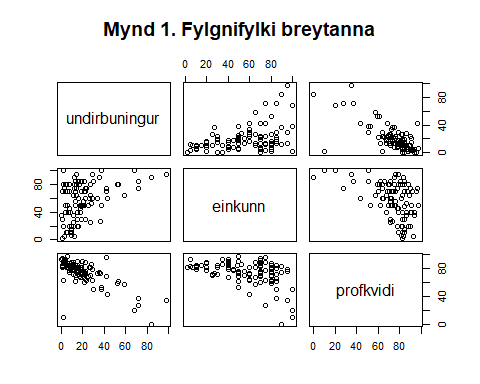
\includegraphics[width=0.5\linewidth]{LengraVerkefni1_files/figure-latex/unnamed-chunk-6-1}
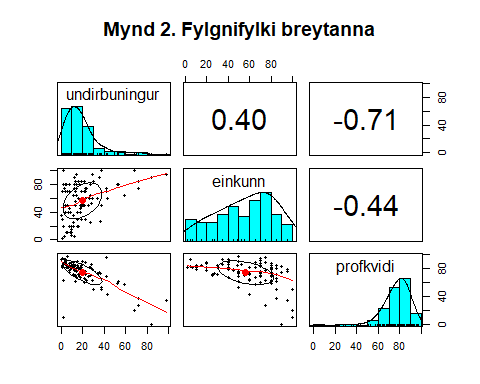
\includegraphics[width=0.5\linewidth]{LengraVerkefni1_files/figure-latex/unnamed-chunk-6-2}

Á myndunum má sjá upplýsingar um dreifingu breytanna og fylgni á milli
þeirra. Dreifing undirbúnings er jákvætt skekkt en flestir nemendur voru
að eyða á bilinu 0 til 35 klukkustundum í undirbúningi fyrir próf.
Einkunnir nemenda nálgast normaldreifingu en flestir nemendur fengu um
60 til 80 stig af 100 mögulegum. Dreifing prófkvíða nemenda var neikvætt
skekkt og á myndinni má sjá að prófkvíði mældist nokkuð hár Flestir
nemendur fengu í kringum 80 stig á \emph{Exam Anxiety Questionnaire}.
Fylgni á milli einkunnar og undirbúnings var meðalhá og jákvæð, 0.40, en
töluverð frávik voru til staðar í undirbúningi eftir því sem einkunn
hækkar. Neikvæð fylgni var á milli prófkvíða og einkunnar, -0.44, og
voru töluverð frávik til staðar í einkunnum, sérstaklega þar sem
prófkvíði var sem mestur. Há neikvæð fylgni mældist á milli prófkvíða og
undirbúnings fyrir próf, -0.71, og voru til staðar frávik sem jukust þar
sem prófkvíði var hæstur.

Framkvæmd var einföld aðfallsgreining þar sem spáð var fyrir um einkunn
nemanda á prófi út frá prófkvíða.

\begin{Shaded}
\begin{Highlighting}[]
\NormalTok{lm.fit }\OtherTok{\textless{}{-}} \FunctionTok{lm}\NormalTok{(einkunn}\SpecialCharTok{\textasciitilde{}}\NormalTok{profkvidi, }\AttributeTok{data =}\NormalTok{ nyttdf)}
\FunctionTok{summary}\NormalTok{(lm.fit)}
\end{Highlighting}
\end{Shaded}

\begin{verbatim}
## 
## Call:
## lm(formula = einkunn ~ profkvidi, data = nyttdf)
## 
## Residuals:
##     Min      1Q  Median      3Q     Max 
## -49.297 -15.373   1.727  20.202  41.557 
## 
## Coefficients:
##             Estimate Std. Error t value Pr(>|t|)    
## (Intercept) 106.0706    10.2855  10.313  < 2e-16 ***
## profkvidi    -0.6658     0.1348  -4.938 3.13e-06 ***
## ---
## Signif. codes:  0 '***' 0.001 '**' 0.01 '*' 0.05 '.' 0.1 ' ' 1
## 
## Residual standard error: 23.4 on 101 degrees of freedom
## Multiple R-squared:  0.1945, Adjusted R-squared:  0.1865 
## F-statistic: 24.38 on 1 and 101 DF,  p-value: 3.128e-06
\end{verbatim}

\begin{Shaded}
\begin{Highlighting}[]
\NormalTok{car}\SpecialCharTok{::}\FunctionTok{Confint}\NormalTok{(lm.fit)}
\end{Highlighting}
\end{Shaded}

\begin{verbatim}
##                Estimate      2.5 %      97.5 %
## (Intercept) 106.0705895 85.6669488 126.4742303
## profkvidi    -0.6657968 -0.9332643  -0.3983292
\end{verbatim}

Frumbreytan prófkvíði spáir marktækt fyrir um einkunn með \emph{p} =
\ensuremath{3.1278728\times 10^{-6}} sem er minna en \(\alpha = 0,05\).
Skurðpunktur fyrir prófkvíða er 106.07 og hallastuðullinn er -0.67.
Hallastuðullinn gefur til kynna að fyrir hvert stig sem nemandi fær á
prófkvíðaskalanum þá lækkar einkunn nemanda á prófi um 0.67.
Öryggisbilið sýnir að sú lækkun geti verið á bilinu 0.93 til 0.40,
ÖB{[}-0.93;-0.40{]}. Skýringarhlutfallið var 18,65\%, sem segir að
18,65\% af heildarbreytileika einkunnar má skýra með breytingum á
prófkvíða.

\begin{Shaded}
\begin{Highlighting}[]
\FunctionTok{plot}\NormalTok{(einkunn}\SpecialCharTok{\textasciitilde{}}\NormalTok{profkvidi, }\AttributeTok{data =}\NormalTok{ nyttdf, }\AttributeTok{xlab=}\StringTok{"Prófkvíði"}\NormalTok{, }\AttributeTok{ylab=}\StringTok{"Einkunn"}\NormalTok{, }\AttributeTok{main=}\StringTok{"Mynd 3. Fylgnirit  einkunna og prófkvíða"}\NormalTok{)}
\FunctionTok{abline}\NormalTok{(lm.fit, }\AttributeTok{lwd =} \DecValTok{2}\NormalTok{, }\AttributeTok{col=}\StringTok{"red"}\NormalTok{)}
\FunctionTok{grid}\NormalTok{()}
\end{Highlighting}
\end{Shaded}

\includegraphics{LengraVerkefni1_files/figure-latex/unnamed-chunk-8-1.pdf}

Á myndritinu má sjá neikvæða fylgni á milli prófkvíða og einkunna. Það
þýðir að því meiri prófkvíða sem nemandi var með, því lægri var einkunn
nemanda á prófi. Það voru smávægileg frávik á einkunnum þegar prófkvíði
var lægstur en það jókst síðan töluvert eftir því sem prófkvíði hækkaði.
Mestu frávikin voru í kringum 80 stig en flestir nemendur voru að skora
á því bili á prófkvíðakvarðanum. Línan gefur þó til kynna að einkunn
lækki að jafnaði eftir því sem prófkvíði hækkar.

\hypertarget{umruxe6uxf0a}{%
\section{Umræða}\label{umruxe6uxf0a}}

Markmið rannsóknarinnar var að kanna hvort prófkvíði væri vandi sem væri
til staðar og hver áhrif kvíðans væru. Það var gert með því að mæla
prófkvíða með \emph{Exam Anxiety Questionnaire}, mæla tíma sem nemendur
eyða í undirbúning fyrir próf og einkunnir á prófi. Niðurstöðurnar gefa
til kynna að prófkvíði sé raunverulegur vandi sem hafi áhrif á
einkunnir. Það má til að mynda sjá út frá meðaltali nemenda á
prófkvíðaskalanum, sem var nokkuð hátt eða 74.34. Mynd 2 sýndi einnig að
flestir nemendur væru að fá í kringum 80 stig af 100 mögulegum á
skalanum. Það má því álykta að margir nemendur upplifi prófkvíða sem
sýnir að vandinn sé til staðar.

Einhliða aðfallsgreining sýndi að eftir því sem prófkvíði eykst þá
bitnar það á einkunum nemenda. Aðfallsgreining sýndi að einkunn lækki um
0.67 stig. Út frá þessum niðurstöðum má gera ráð fyrir því að því meiri
sem prófkvíði nemanda er því lægri einkunnir fær sá nemandi. Frávik voru
þó til staðar á fylgniriti sem sýnir að prófkvíðinn hafi ólík áhrif á
nemendur. Nokkrir nemendur voru að fá hærri einkunn en forspá gaf til
kynna um þó þeir hafi skorað hátt á prófkvíðakvarðanum. Það má álykta að
prófkvíði hafi ekki endilega hamlandi áhrif á þá nemendur. Nokkrir aðrir
nemendur voru þó að fá lægri einkunn en forspá gaf til kynna um sem
sýnir að þetta geti verið hamlandi vandi og komið niður á einkunnum
nemenda. Þar af leiðandi er ekki hægt að álykta um að þetta sé ekki
raunverulegur vandi þó frávik hafi verið til staðar.

Það er því gríðarlega mikilvægt að veita viðeigandi inngrip við þessum
vanda svo nemendur geta nýtt færni sýna að fullnustu í námi án þess að
upplifa nokkurs konar hömlur. Næstu skref væru að nýta aðstoðina sem
fyrirtækið veitir og sigrast á eða minnka prófkvíðann sem er til staðar.

\end{document}
